\documentclass{article}
\usepackage{graphicx}
\usepackage{tabularx}
\usepackage{float}
\usepackage[width=18cm, height = 25cm]{geometry}

\title{Work report 140222: Co-sputtered ZnO-SnO$_2$}
\author{Rob Treharne}

\begin{document}

\maketitle

\section{Overview}

Samples for Binghampton. Co-sputtered ZTO films on conductive substrates.


\section{Samples}

\begin{table}[h!]
\caption{Sample deposition parameters. Both films are deposited on 1mm thick aluminaborosilicate glass (ABS) substrates coated with a $250$ nm thick film of ITO ($10$ $\Omega/$square).}
\centering
\begin{tabular}{l|cc}
\hline\hline
 ID & 140516\_2 & 140519\_2 \\
\hline
Material & ZnO:SnO$_2$ & ZnO:SnO$_2$ \\
RF power (W) & 250:80 & 70:80 \\
Ar pressure (mTorr) & 5 & 5 \\
dep. time (min) & 30 & 30 \\
T$_{dep}$ ($^{\circ}$C) & 18 & 18 \\
\hline
\end{tabular}
\end{table}




\section{Film profiles}

\begin{figure}[ht]
\centering
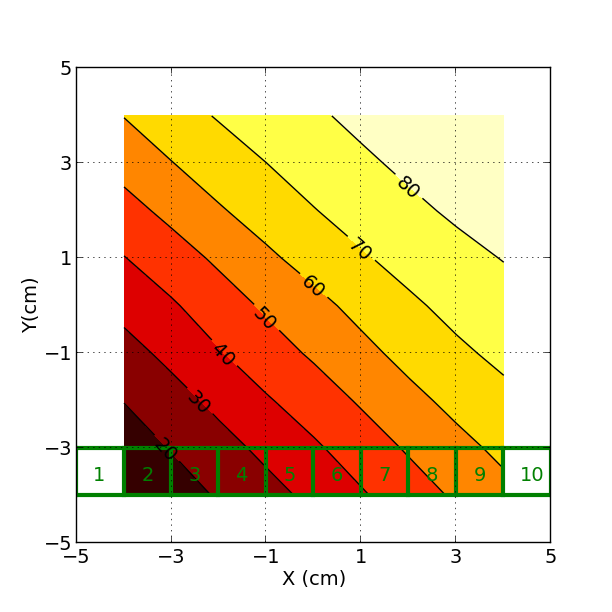
\includegraphics[width=0.5\textwidth]{140519_2_ZnO_SnO2_pieces_250-80.png}
\caption{\label{fig:3} 140516\_2\_ZnO\_SnO$_2$: $\%$ wt. SnO$_2$ profile of co-sputtered film. Green sample series cut from sample.}
\end{figure}

\begin{figure}[ht]
\centering
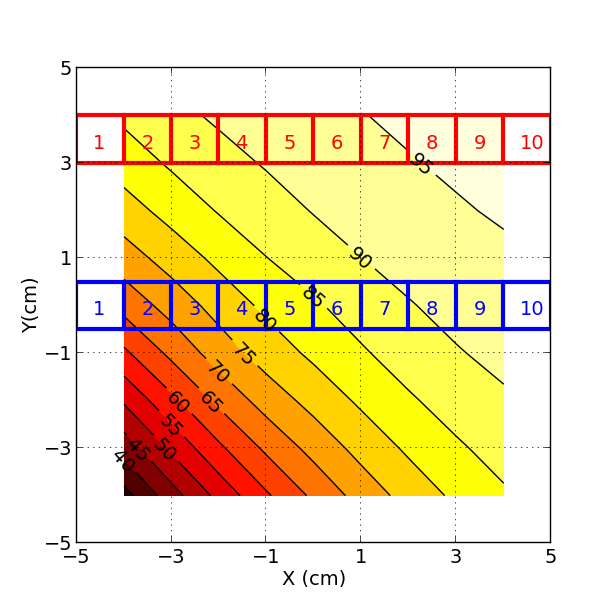
\includegraphics[width=0.5\textwidth]{140519_2_ZnO_SnO2_pieces.png}
\caption{\label{fig:3} 140519\_2\_ZnO\_SnO$_2$: $\%$ wt. SnO$_2$ profile of co-sputtered film. Red and blue sample series cut from sample.}
\end{figure}



\begin{table}[p]
\caption{Aporoximate $\%$ wt. SnO$_2$ content for green, red and blue sample series cut from ZTO samples.}
% title of Table
\centering
% used for centering table
\begin{tabular}{c c c c}
% centered columns (4 columns)
\hline\hline
%inserts double horizontal lines
Piece & Green & Red & Blue  \\ [0.5ex]
% inserts table
%heading
\hline
% inserts single horizontal line
1 & 9.8 & 81.0 & 60.0  \\
2 & 15.3 & 84.1 & 66.2  \\
3 & 21.0 & 87.0 & 71.7  \\
4 & 26.8 & 89.3 & 76.6  \\
5 & 32.6 & 91.3 & 80.9 \\
6 & 38.6 & 93.0 & 84.4  \\
7 & 44.7 & 94.3 & 87.4  \\
8 & 50.9 & 95.3 & 89.6  \\
9 & 57.2 & 95.9 & 91.2 \\
10 & 63.6 & 96.0 & 92.2  \\
% [1ex] adds vertical space
\hline
%inserts single line
\end{tabular}
\label{table:nonlin}
% is used to refer this table in the text
\end{table}






\end{document}